\documentclass[10pt]{beamer}

\usetheme{metropolis}
\usepackage{appendixnumberbeamer}
\usepackage{bm}
\usepackage{booktabs}
\usepackage[scale=2]{ccicons}

\usepackage{pgfplots}
\usepgfplotslibrary{dateplot}

\usepackage{xspace}
\newcommand{\themename}{\textbf{\textsc{metropolis}}\xspace}

\title{Statistical Modelling of Induced Earthquakes}
\subtitle{Thesis presentation}
\date{Friday $24^{\text{th}}$ September 24, 2021}
\author{Zak Varty}
\institute{STOR-i CDT, Lancaster University}
% \titlegraphic{\hfill
\includegraphics[height=1.5cm]{logo.pdf}}

\begin{document}

\maketitle

\section{Motivation and Aims}


\begin{frame}{Motivations}
\begin{center}
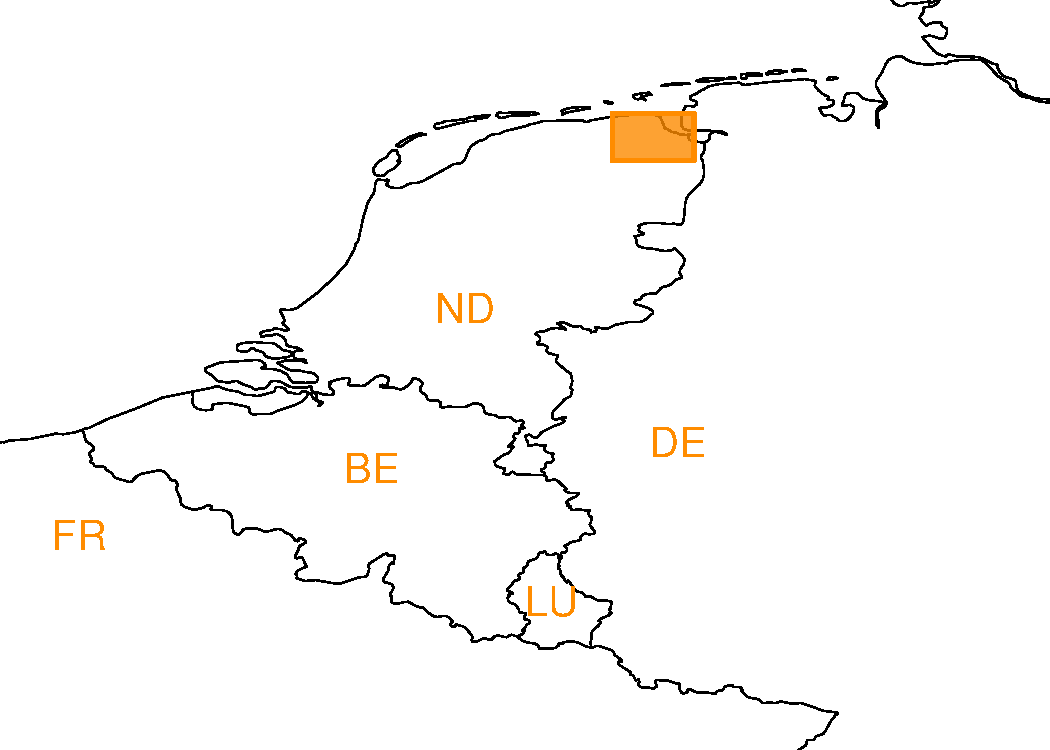
\includegraphics[width = 0.4\textwidth]{Groningen_window_europeII.pdf}
\end{center}

\begin{itemize}
    \item Earthquakes caused by gas extraction in Groningen. \\[1em]
\item Induced earthquakes: fewer, smaller, changing. \\[1em] 
\item Developing  landscape: gas extraction, sensor network, opinion.  \\[1em]
\end{itemize}
\end{frame}


\begin{frame}{Aims}
     \textbf{Scientific and Industrial}
     \begin{itemize}
         \item {\large1| } Better understand and describe induced earthquakes to inform policy. 
     \end{itemize}
     
     \vspace{2em}
     
     \textbf{Statistical}
     \begin{itemize}
         \item {\large2| } To make better use of the data that \textit{are} available to us .
         \item[]
         \item {\large3| } To improve and extend existing methodology used in seismology. 
     \end{itemize}
\end{frame} 

\section{Contributions \& Impact}

\begin{frame}{Ch 4: Earthquake locations}
\textit{\color{orange} Aim 1: Scientific and Industrial Impact}

\textbf{Contributions:}
Exploratory analysis of physiscal features included and missed from physically motivated model

\vspace{1em}

$$ \lambda(x,t; \bm{\beta}, \bm{s}) = \beta_0 \dot s(x,y)[1 + \beta_1 s(x,t)]\exp\{\beta_1 s(x,t)\} $$

\vspace{2em}

\begin{itemize}
    \item (+) Exp term dominant but linear simplifies interpretation 
    \item (+) Evidence of spatial variability in effect of ICS 
    \item (-) Insufficient evidence of: lag, shift, NFR or smoothing effects. 
\end{itemize}
\end{frame}



\begin{frame}{Ch 4: Earthquake locations}

\textbf{Outcomes:}

\vspace{2em}

Provided empirical evidence toward scientific debate: whose first principles are right? 

\vspace{2em}

Motivated funding for further work into more advanced spatial modelling.

\end{frame}



\begin{frame}{Ch 5: Threshold selection}
\textit{\color{orange} Aim 2: making best use of available data} 

Sensor network changing over time as well as gas extraction: can / should we use additional small EQs?

\vspace{1em}
\textbf{Contributions:}

\begin{itemize}
\item Reframed G-R law as special case of GPD, extending model class; 
\item Novel method for selecting time-varying threshold for extreme value analysis; 
\item Addressing issues with rounded data and partial censoring of small values; 
\item Demonstrated inclusion of small events is beneficial to estimating distribution of large events. 
\end{itemize}

\end{frame}



\begin{frame}{Ch 5: Threshold selection}
\begin{columns}
\begin{column}{0.6\textwidth}
\textbf{Outcomes:} 
\vspace{1em}
\begin{itemize}
\item First method for selecting time varying modelling threshold; \\[1em]
\item More than doubled data usage;\\[1em]
\item Empirical evidence that $\xi_m < 0$; \\[1em]
\item Justifies investment in EQ detection; \\[1em]
\item Further work on stability and impact of choice of measurement scale. 
\end{itemize}
\end{column}
\begin{column}{0.4\textwidth}
\begin{center}
    \includegraphics[width = \textwidth, page = 2]{BO_selected_thresholds_restricted.pdf}
    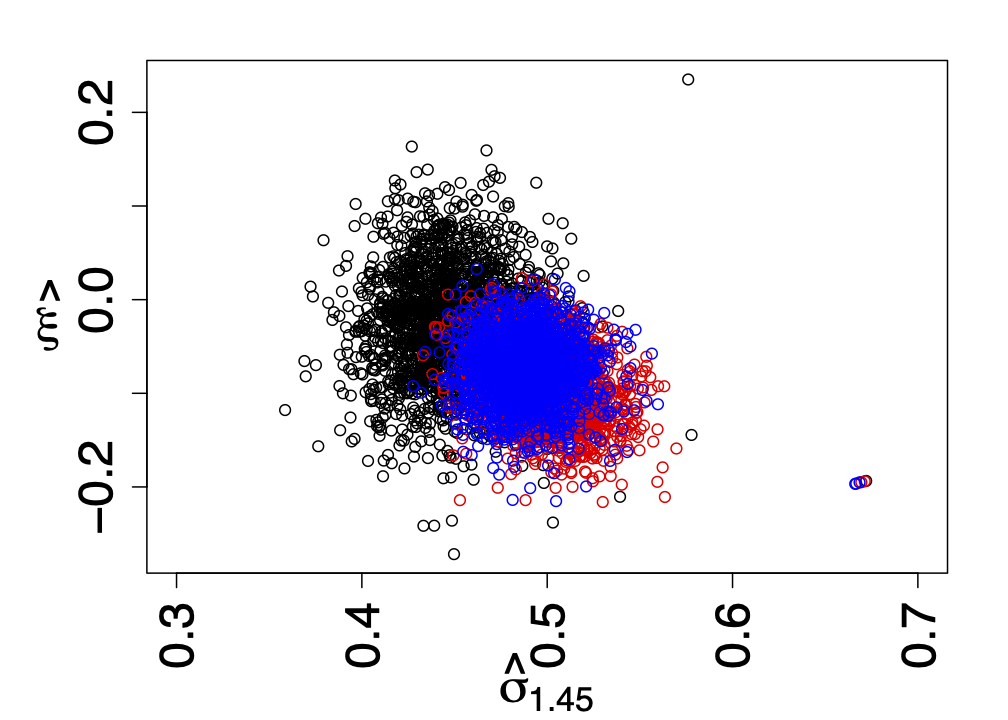
\includegraphics[width = \textwidth]{parameter_comparison_cons_flat_sigmoid.png}
\end{center}
\end{column}
\end{columns}
\end{frame}



\begin{frame}{Ch 6: Improving and extending ETAS}
\textit{\color{orange} Aim 3: Improve and extend seismological models} 

ETAS assumes IID magnitudes and is difficult to fit directly. How can we improve using conditional inference methods? 

\vspace{1em}
\textbf{Contributions:} 
\begin{itemize}
\item Empirical laws: really just a GPD or a GLM.  Demonstrated that reparameterisation generalises and improves inference. 
\item Relaxing assumptions: Developed models, inference methods and testing for dual and correlated magnitudes.
\item Investigated for the first time branching vector recovery. 
\end{itemize}
\end{frame}



\begin{frame}{Ch 6: Improving and extending ETAS}
\textbf{Outcomes:}
\begin{itemize}
    \item Motivated use of GPD and conditional inference in physical models;\\[1em]
    \item Nudged seismologists toward EVT methods; \\[1em]
    \item beta-version of R package to promote practitioner use;\\[1em]
    \item Lays foundations for further work exploring dual and dependent magnitudes .
\end{itemize}
\end{frame}



\section{Limitations and Further work}

\begin{frame}{Limitations}
    
\textbf{Ch 4:} in-sample testing, limited power, alternative models for same physical features.

\vspace{2em}

\textbf{Ch 5:} Temporal only, computationally intensive, heuristic, application-methodology middle-ground. 

\vspace{2em}

\textbf{Ch 6:} (extensions) Temporal only, stationary background, Gaussian copula, accessibility to seismologists.
\end{frame}



\begin{frame}{Further Work}
 \textbf{I'm out of time but there is so much still to do!}

\begin{itemize}
    \item Draw together results from different chapters: e.g. include small events in physical models, spatial modelling threshold or ETAS extensions. 
    \item [] 
    \item Comparison to other threshold selection methods in standard EVT setting.  
    \item []
    \item Dual / corr model with non-constant seeding using, e.g. parametric or (thin-plate) spline model. 
\end{itemize}
\end{frame}

\section*{Thank you for your time,\\ any questions?}
\end{document} 